\documentclass[12pt]{report}
\usepackage[margin=1in]{geometry}
\usepackage{graphicx}

\begin{document}

\begin{center}
\begin{Large}
\textbf{
	DIMENSIONAL ANALYSIS OF FASTENERS USING MACHINE VISION
}
\end{Large}
\end{center}

\begin{large}
\begin{center}
\textbf{
	Phase I: Progress
}
\end{center}
\end{large}

The hardware mainly consists of the raspberry pi micro-controller, a stepper motor, a camera, a line laser and a rotating platform housed in a container.

The camera is connected to a special camera port present on the raspberry pi and can be easily controlled by using a Python module (\emph{picamera}). The focus of the camera is adjustable and is set to correspond to the distance between the camera and the center of the platform. It was found that a near focused image provided better details than a camera focused at infinity.

The line laser is a 5mW 650nm laser module which is driven by a transistor(its name) controlled by the pi. The smallest size measurable from the laser profile depends mainly on the thickness of the laser. Thinner laser line yields a better detail of the nut/bolt. But that decreases the brightness of the laser, which may not be detected by the camera.
\begin{figure}[h]
\centering
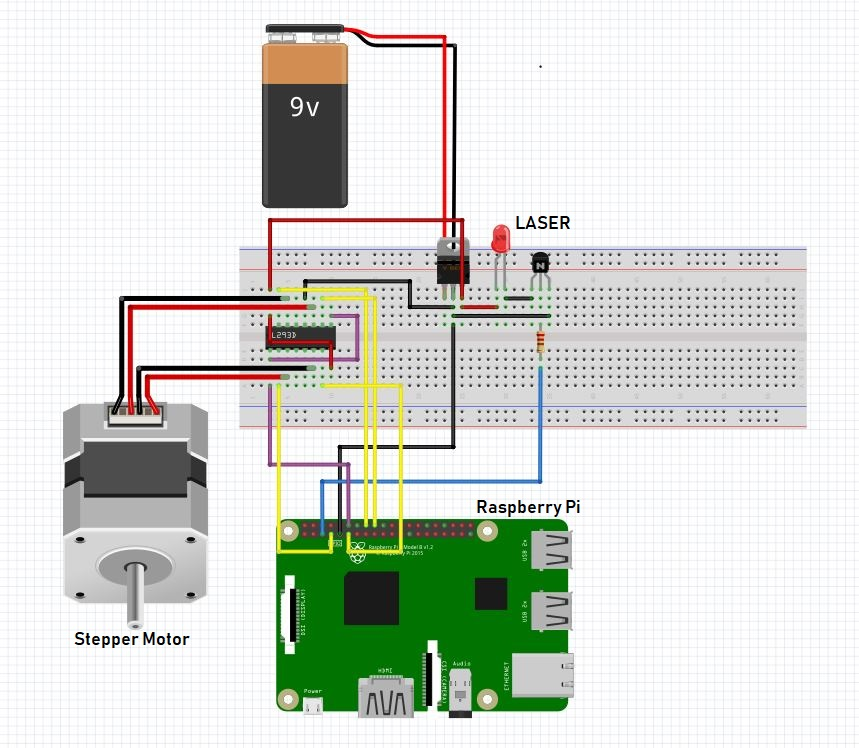
\includegraphics[scale=.5]{circuit.jpg}
\caption{Circuit}
\end{figure}
The stepper motor used here is 28BYJ-48. The stepper motor is driven by the L293D driver IC, connected to the pi. Since the load on the motor shaft is axial and not radial, the motor does not require too much torque to rotate the platform with the fastener on it. Hence a small stepper motor sufficed for our purposes. The maximum number of steps the stepper motor can rotate to complete one revolution is $512$. This means we can atmost take $512$ unique images of the laser profiled bolts/nuts for a single rotation. This corresponds to a resolution of $0.703\deg$. We can adjust the angle of rotation of the platform by specifying the number of steps the motor has to rotate before stopping.
The laser is then turned on the fastener and an image of the fastener is taken by the camera and stored in the memory. Decreasing the angle of rotation between each image taken increases the details captured but also increases the processing of those images, affecting either performance or speed of execution.\\
%Circuit Image
\begin{figure}[h]
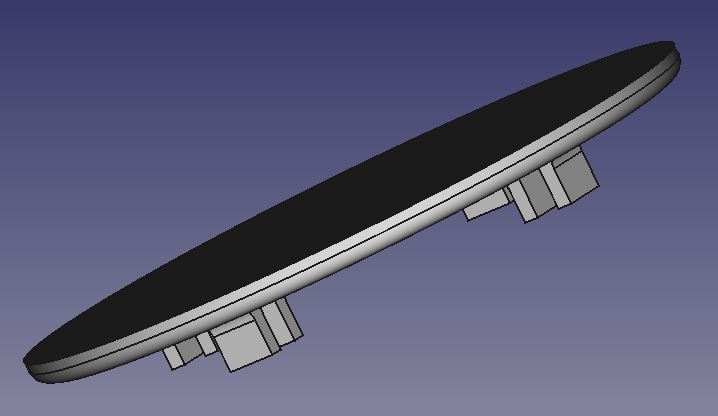
\includegraphics[scale=0.3]{platform_top.jpg}
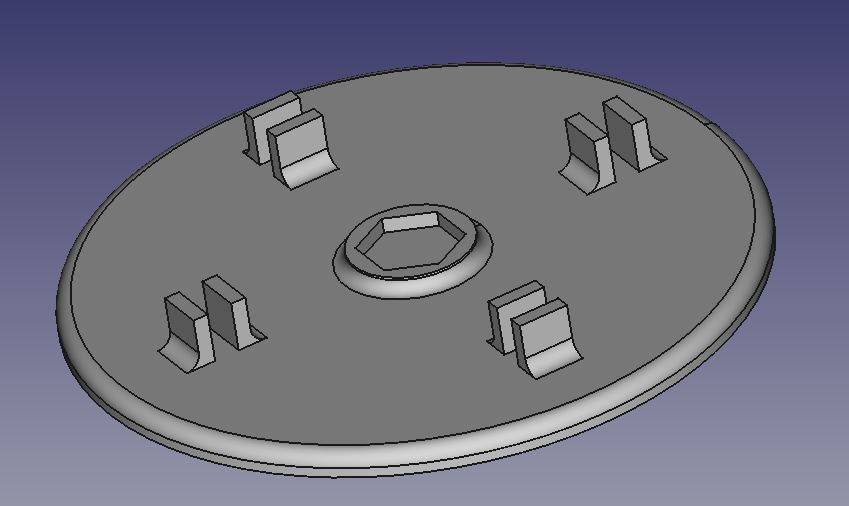
\includegraphics[scale=0.25]{platform_bottom.jpg}
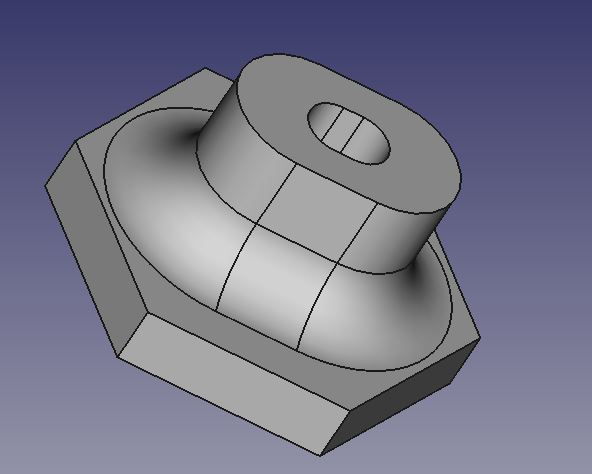
\includegraphics[scale=0.3]{connector.jpg}
\caption{3D Model of the platform}
\end{figure}

Initially, the platform was created in thick cardboard sheets. But the cardboard was not strong enough to hold the weight of the fastener and became unstable. The instability was due to the fact that the only support for the platform was from the shaft of the motor. If the motor was on unstable ground, it resulted in blurred images or toppling of the fastener. Due to a need for a sturdy and lightweight material for the platform, the platform was designed in freeCAD software and created using a 3D printer.
The platform contains two parts: the platform itself and a connector which connects the shaft of the motor to the platform. The model was designed this way so as to have more flexibility in the design. If the motor were to be changed in the future, the whole platform need not be created from scratch; rather, we just need to create a different sized connector and use it with the platform.\\ 
%Dimenisions of the platform
%Image

To start with, images of the bolts were taken in open space. This induced noise in the images and the laser profiles could not be extracted at high precision. The noise was reduced by taking the images in a dark environment. So we used a container to block off stray light incident on the camera. The interior of the container is covered in black to further reduce the background noise.
%Hardware setup image


\newpage
\begin{figure}[h]
\centering
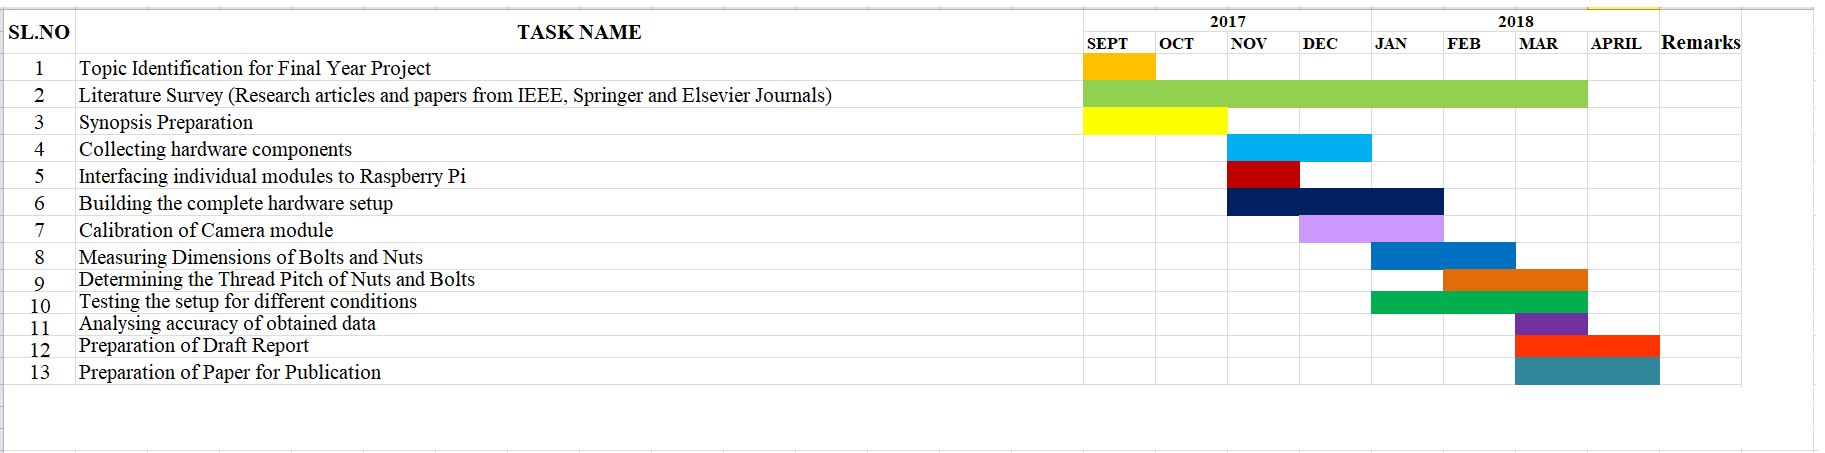
\includegraphics[width=1.3\textwidth, height=0.4\textwidth, angle=90]{pertchart.jpg}
\end{figure}
\end{document}